% !TeX spellcheck = en_US

% Recommended reading:
\begin{frame}
	Recommended reading:
	\begin{itemize}
		\item Lectures 4, 5 in \cite{TreBau}
		\item Sections \texttt{I}.8 and \texttt{I}.9 in \cite{StrangData}
	\end{itemize}
	
	%	\bibliographystyle{plain}
	~\\~\\
	Literature:\\
	\bibliography{../information/literature.bib}
\end{frame}


\begin{frame}
\Section{Singular Values and the Singular Value Decomposition (SVD)}
We will extend the concept of eigenvalues and eigenvectors to general matrices $A \in \Rmn$.\\~\\
\Subsection{Motivation and Introduction}
~\\
\begin{center}
	\textbf{Gilbert Strang:} \textit{``The SVD $A=U\Sigma V^\top$ is the \textbf{most important} theorem in data science.''} \\{\small ~~~~~(\cite{StrangData} Linear Algebra and Learning from Data, p.31)}\\[0.3cm] 
\end{center}
~\\~\\
\textbf{Importance and Applications:}\\
\begin{itemize}
	\item The SVD of a matrix reveals many properties about the matrix itself (representation of the image and kernel, rank, invertibility, condition,...)
	\vspace{0.2cm}\item Low-Rank Approximation
	\begin{itemize}
	\vspace{0.2cm}\item Data compression (e.g., image data)
\vspace{0.2cm}\item Principal Component Analysis 
	\end{itemize}
	\vspace{0.2cm}\item Pseudoinverse (generalization of the inverse matrix) and relation to the minimum-norm least squares solution
\end{itemize}
\end{frame}

\begin{frame}
\textbf{ Image and data compression:}\\	~\\~\\
 \begin{minipage}[c]{0.6\textwidth}
 	
 	\begin{tikzpicture}
 	\node[inner sep=0pt] (dina0) at (0,0)
 	{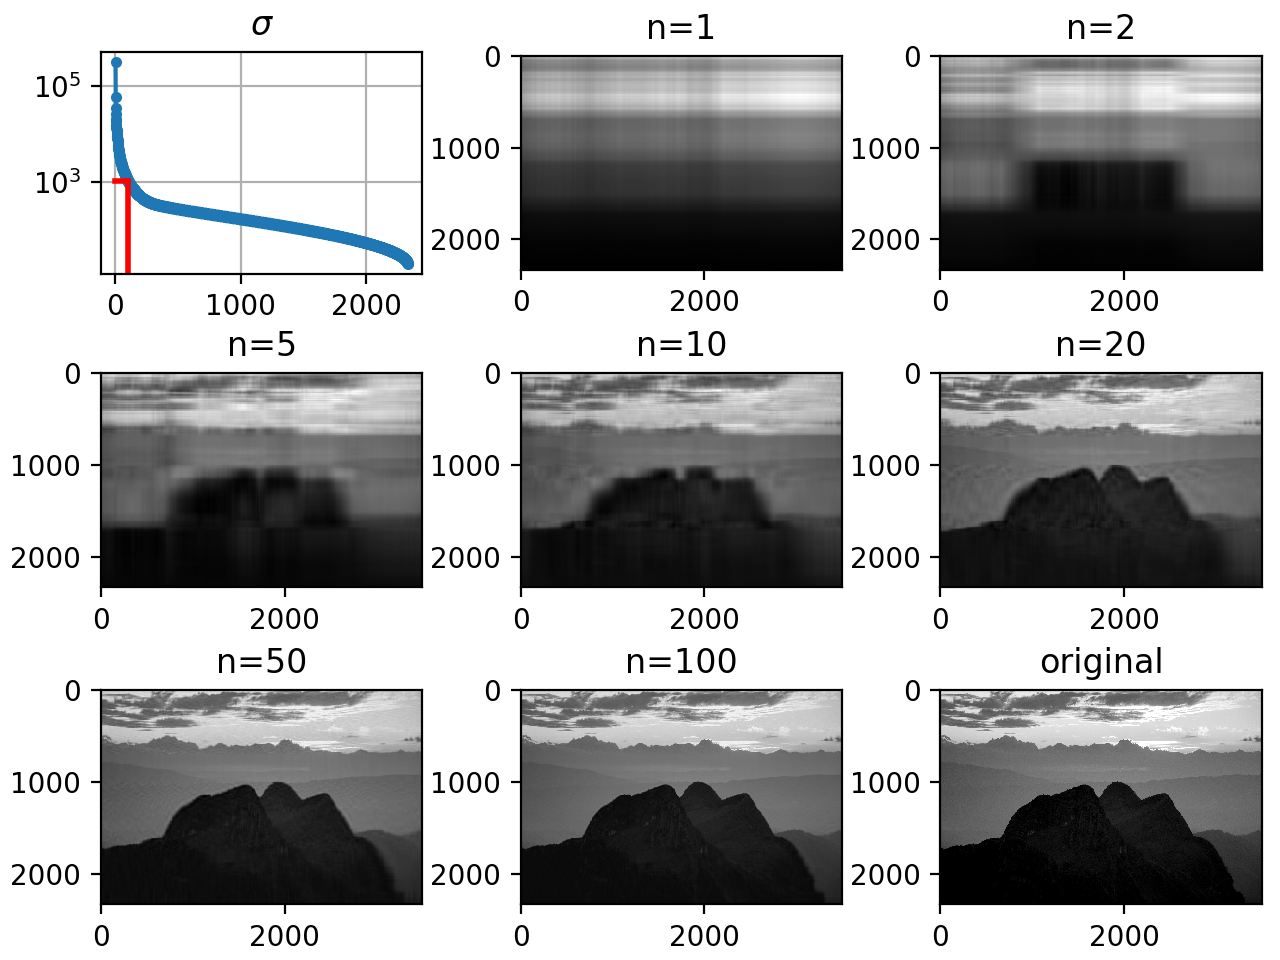
\includegraphics[width=\textwidth]{6_svd_mountain.png}};
 	\end{tikzpicture}	
 \end{minipage}
 \begin{minipage}[c]{0.03\textwidth}
 	\
 \end{minipage}
 \begin{minipage}[c]{0.35\textwidth}
 	$3500\times2333$ greyscale image is interpreted as matrix $$A\in[0,1]^{3500\times2333}.$$ 
 	The singular values are shown in the figure with the title ``$\sigma$''.\\ 
 	The reconstructed image with the first 100 singular values only, i.e.,
 	$$A_{100}:=U\text{diag}(\sigma_1,\ldots,\sigma_{100},0,\ldots ,0)V^\top$$ 
 	is quite close to the original image but takes only
 	\[
 	\frac{3500\cdot 100+100+100\cdot 2333}{3500\cdot 2333}\approx 7\%
 	\]
 	of the storage space.
 \end{minipage}
\end{frame}


\begin{frame}
\textbf{Principal Component Analysis}\\
~\\
 Under the correct setup we have that the SVD equals the PCA, whose aim is dimension reduction:\\~\\
\begin{center}
	\colorbox{white}{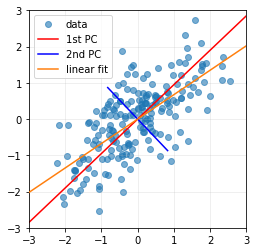
\includegraphics[width=0.4\textwidth]{pca_ex.png}} 
\end{center} 
The data represented by the blue dots can be fully explained by the red and blue line. However the red line might already capture a substantial part of the data's variance.
\end{frame}



% DERIVE SVD
\begin{frame}
\textbf{The Singular Value Decomposition (SVD)}\\
For matrices $A \in \Rmn$ of general format, the equation $Av  = \lambda v$ fails. Instead we define:
\begin{definition}[Singular Values and Vectors]\label{def:singularValVec}
Let $A \in \Rmn$ be a matrix. Then a positive number $\sigma >0$ is called \textit{\textbf{singular value}}, if there exist nonzero vectors $v \in \Rn \setminus \{0\}$ and $u \in \Rm\setminus \{0\}$, such that
\begin{align}
Av = \sigma u ~~~\text{and}~~~A^\top u = \sigma v. \label{eq:SVDstart}
\end{align}
The vectors $v$ and $u$ are called right and left \textit{\textbf{singular vectors of $A$}} to the singular value $\sigma$.
\end{definition}
%
~\\
\Hide{
Assume we had singular vectors $v_i, u_i$ and values $\sigma_i$ and put them into matrices $V, U, \Sigma$ (as we did for the eigendecomposition). Then we find
$$AV = U \Sigma$$% ~~~~(\text{and later also:}~~ A=U\Sigma V^\top) $$
}
~\\~\\
This will lead to the impactful theorem of the singular value decomposition: \vspace*{-0.3cm}
\begin{theo}[Singular value decomposition (SVD)]\label{theo:SVD-exist} Let $A\in\R^{m\times n}$. Then there are orthogonal matrices $U\in\R^{m\times m}$ and $V\in\R^{n\times n}$ as well as a diagonal matrix $\Sigma = \text{diag}(\sigma_1,\ldots, \sigma_r,0,\ldots,0) \in \Rmn$, where $\sigma_1\ge\sigma_2\ge\ldots\ge\sigma_r> 0\, ,\ r \leq\min\{m,n\}$, are the sorted positive singular values, such that 
	$$A=U \Sigma V^\top,$$
	which is the	so-called \textit{\textbf{singular value decomposition of $A$}} .
\end{theo}
\end{frame}


\begin{frame}
\Subsection{Preparing Results}	
In order to understand and prove this central theorem we will put a few auxiliary results into position. The first one is about eigenvalues of symmetric and positive semi-definite matrices:
\begin{lemma}[Eigenvalues and Positivity] \label{lem:eigvalsPositivity}
	Let $B \in \Rnn$ be symmetric and positive definite (semi-definite), then $\lambda > 0$ ($\geq 0$) for all eigenvalues $\lambda \in \sigma(B)$.
\end{lemma}
\Hide{ 
	\begin{proof}
		First of all we note that due to symmetry $\sigma(B) \subset \R$ and we can choose eigenvectors with real coefficients.\\
		 We now perform a proof by contradiction:\\
		Let $B$ be $\underbrace{\text{positive definite}}_{\textcolor{cyan}{:\Leftrightarrow x^\top Bx>0~\forall x\neq 0}}$ and assume $\lambda\leq0$ for some $\underbrace{\lambda\in\sigma(B)}_{\textcolor{cyan}{:\Leftrightarrow \exists v\neq 0: Bv=\lambda v}}$ with eigenvector $v \in \Rn, v\neq 0$.\\
Then we find
$$
v^\top \underbrace{Bv}_{\textcolor{cyan}{=\lambda v}} 
= \lambda v^\top v
= \underbrace{\lambda}_{\textcolor{cyan}{\leq0}}\underbrace{\|{v}\|_2^2}_{\textcolor{cyan}{>0}} ~\leq 0~ ~~~\textcolor{red}{\text{[contradiction to the positivity of A]}}.$$

(Analogous proof for $B$ positive semi-definite.)\\
(Alternative proof via Rayleigh quotient.)\\
%	Let $A$ be positive definite (semi--definite) and let $(\lambda, v)$ be an eigenpair of $A$. Then by using the Rayleigh quotient we find
%$$\lambda = \frac{v^\top A v}{v^\top v} = \frac{v^\top A v}{\|v\|_2^2}~~{\color{cyan}\tfrac{> 0~~ (\geq 0)}{> 0 ~ \text{since}~v\neq 0  }} ~~> 0~~ (\geq 0). $$
\end{proof}
}

\end{frame}
\begin{frame}
The next result is about the shared eigenvalues of product matrices:\\
\begin{lemma}[Shared Eigenvalues of Products] \label{lem:eigvalsProducts}
	Let $A\in \F^{m \times n}$ and $B \in \F^{n \times m}$. Then the products $AB \in \F^{m \times m}$ and $BA \in \Fnn$ have the same \underline{nonzero} eigenvalues.
\end{lemma}
\Hide{
	\begin{proof}
	We prove this by mutual subset relation:\\
	First let $\lambda \in \sigma(AB), \lambda \neq 0$ be a nonzero eigenvalue of $AB$ with eigenvector $v \in \F^n, v \neq 0$, i.e., $$ABv = \lambda v.$$ Now multiply both sides by $B$ to obtain $$BA(Bv) = \lambda Bv, $$
	which implies that $Bv$ is an eigenvector of $BA$ with the \textit{same} eigenvalue $\lambda$. To see this, note that $\lambda \neq 0$ implies that $ABv = \lambda v \neq 0$ and thus $Bv \neq 0$.\\~\\
	Similarly, let now $\lambda \in \sigma(BA), \lambda \neq 0$ be a nonzero eigenvalue of $BA$ with eigenvector $v \in \F^n, v \neq 0$, i.e., $BAv = \lambda v$. Then we multiply both sides by $A$ to proceed along the same lines.
	\end{proof}
~\\
}
Remark: 
\begin{itemize}
	\item If $m\neq n$, then $BA$ and $AB$ have differently many eigenvalues. However the nonzero eigenvalues are the same. Thus both product matrices have at most $\ell := \min\{m,n\}$ nonzero eigenvalues!
	\item In the special case that $m=n$ and $B$ invertible, we observe $$B^{-1}(BA)B = (AB), $$
	identifying the matrices $AB$ and $BA$ as being similar!
\end{itemize}
\end{frame}
 
 
\begin{frame}
Now a special instance of the latter two results (choosing $B=A^\top$) leads us to the key lemma to prove the SVD Theorem \ref{theo:SVD-exist}: \vspace{-0.1cm}
\begin{lemma} \label{lem:eigenvalues_of_products}
	Let $A \in \Rmn$, then the matrices $A^\top A$ and $AA^\top $ are symmetric, positive semi-definite and have the same positive eigenvalues.
\end{lemma}
\Hide{
\begin{proof}We find:
	\begin{itemize} 
		\item [ 1)]
		\underline{Symmetry:} $(A^\top A)^\top = A^\top (A^\top)^\top = A^\top A$ and similarly $(AA^\top )^\top =AA^\top $
		\item [ 2)]
		\underline{p(s)d:} $x^\top A^\top Ax=\|Ax\|_2^2\geq 0,~~~x^\top AA^\top x=\|A^\top x\|_2^2\geq 0$
		\item [ 3)] The same positive eigenvalues:
		\begin{itemize}
			\item[ -] By Lemma \ref{lem:eigvalsPositivity} we know that the matrices only have nonnegative eigenvalues
			\item[ -] By lemma \ref{lem:eigvalsProducts} we know that the nonzero, i.e., positive, eigenvalues are the same
		\end{itemize}
	\end{itemize}
\end{proof} }
~\\
\textbf{Remark:} ~\\Due to the symmetry of $A^\top A$ and $AA^\top $ we also know that we find \underline{orthonormal} eigenvectors $v_1,\ldots, v_n$ and $u_1,\ldots, u_m$! The SVD will connect them!
\end{frame}


%%%%%
% proof SVD short
%%%
\begin{frame}
	\Subsection{From Reduced to Full SVD}
\Hide{	\scriptsize
	Recall:\\
	\begin{itemize}\scriptsize
		\item $\im(A) \perp \ker(A^\top)$ and $\im(A^\top) \perp \ker(A)$
		\item $A^\top A$, $AA^\top$ are
		\begin{itemize}\scriptsize
			\item symmetric $\Rightarrow$ real eigenvalues and we find orthonormal basis of eigenvectors
			\item positive semi-definite  $\Rightarrow$ their eigenvalues are nonnegative, i.e., $\lambda \geq 0$
			\item they have the \textit{same} positive eigenvalues $\lambda_i$ for $1\leq i \leq r \leq \min(m,n)$
			\item $\ker(A)=\ker(A^\top A)$ and $\ker(A^\top)=\ker(AA^\top)$
		\end{itemize}
	\end{itemize}
~\\
	\textbf{Proof of SVD}: We are looking for nonzero vectors $u\in\Rm, v\in\Rn$ and positive numbers $\sigma>0$, such that
	\begin{align}
	Av &= \sigma u ~~~\iff  ~~u=\frac{1}{\sigma}Av\in \im(A)\label{eq:singDef1},\\
	A^\top u &= \sigma v~~~\iff v=\frac{1}{\sigma}A^\top u \in \im(A^\top) \label{eq:singDef2}.
	\end{align}
	\textbf{1)} So we have two equations for two unknown vectors. By inserting one into the other we obtain two equivalent formulations (this is \textit{elimination}). Here, we insert \eqref{eq:singDef1} into \eqref{eq:singDef2} which gives
	\begin{align}
	A^\top Av = \sigma^2 v ~~ \iff ~~( \sigma^2,v) ~\text{eigenpair of}~A^\top A .\label{eq:SVDrecipe}
	\end{align}
	(Note: Inserting \eqref{eq:singDef2} into \eqref{eq:singDef1} would give $( \sigma^2,u) ~\text{eigenpair of}~A A^\top$)\\
	\textbf{2)} Let $\lambda_1,\dots,\lambda_r>0~(r\leq\min(m,n))$ be the positive eigenvalues of $A^\top A$ with orthonormal eigenvectors $v_1,\dots,v_r$ ($\in \im(A^\top)$). Then according to \eqref{eq:singDef1} and \eqref{eq:SVDrecipe} we set
	$$
	\sigma_i:=\sqrt{\lambda_i},~~~~u_i:=\frac{1}{\sigma_i}Av_i~(\in \im(A)).
	$$
	We then find:
	\begin{itemize}\scriptsize
		\item By construction $v_i, u_i$ are singular vectors to the singular value $\sigma_i$, i.e., we have
		$$Av_i=\sigma_iu_i$$
		\item [] and indeed %we find that
		$$A^\top u_i=\frac{1}{\sigma_i}\underbrace{A^\top Av_i}_{=\lambda_iv_i}=\frac{\lambda_i}{\sigma_i}v_i=\sigma_iv_i.$$
		\item For the SVD we want the $u_i$ to be orthonormal. Let us check this:
		$$u_i^\top u_j=\frac{1}{\sigma_i}\frac{1}{\sigma_j}(Av_i)^\top Av_j=\frac{1}{\sigma_i}\frac{1}{\sigma_j}v_i^\top \underbrace{A^\top Av_j}_{=\lambda_jv_j}=\underbrace{\frac{\sigma_j}{\sigma_i}}_{\neq 0}\underbrace{v_i^\top v_j}_{=\delta_{ij}}=\delta_{ij}.$$
	\end{itemize}}
\end{frame}
\begin{frame}
\Hide{	\footnotesize
	\textbf{3)} Finally, choose orthonormal bases 
	\begin{align*}
	v_{r+1},\ldots, v_{n} &\in  \ker(A)~~(\perp\im(A^\top)), \\
	u_{r+1},\ldots, u_{m} &\in  \ker(A^\top)~~(\perp\im(A)) .
	\end{align*}
	We note that these are eigenvectors of $A^\top A$ and $AA^\top$, respectively, to the eigenvalue $0$.
	Then let us collect everything:
	\begin{align*}
	V:=\left(
	\underbrace{\begin{matrix}
		|&~&|\\v_1&\cdots&v_r\\|&~&|
		\end{matrix}}_{= V_r,~\in\text{Im}(A^\top) }
	\underbrace{\begin{matrix}
		|&~&|\\v_{r+1}&\cdots&v_n\\|&~&|
		\end{matrix}}_{\in\text{ker}(A)}
	\right)\in\mathbb{R}^{n\times n},~~~
	U:=\left(
	\underbrace{\begin{matrix}
		|&~&|\\u_1&\cdots&u_r\\|&~&|
		\end{matrix}}_{=U_r,~\in\text{Im}(A)}
	\underbrace{\begin{matrix}
		|&~&|\\u_{r+1}&\cdots&u_m\\|&~&|
		\end{matrix}}_{\in\text{ker}(A^\top) }
	\right)\in\mathbb{R}^{m\times m}
	\end{align*}
	$$\Sigma :=\left(\begin{array}{ccc|ccc}
	\sigma_1&&&&\vdots&\\
	&\ddots&&\cdots&0&\cdots\\
	&&\sigma_r&&\vdots&\\\hline
	&\vdots&&&\vdots&\\
	\cdots&0&\cdots&\cdots&0&\cdots\\
	&\vdots&&&\vdots&
	\end{array}\right) \in \Rmn .$$
	With $\Sigma_r := \text{diag}(\sigma_1,\ldots,\sigma_r)$ we can write
	\begin{align*}
	AV = (AV_r | 0) = (U_r \Sigma_r | 0) = U\Sigma .
	\end{align*}
	Now, since $V\in\Rnn$ is orthogonal (i.e., $V^{-1} = V^\top$), we can multiply with $V^\top$ from the right and finally obtain the desired SVD 
	$$A = U\Sigma V^\top .$$
%	Due to the zeroes in $\Sigma$ we can also write it in reduced form as 
%	$$ A = U_r\Sigma_r V_r^\top .$$
	~\\
	Remark: The zeros in $\Sigma$ may justify to also allow for zero singular values $\sigma_{r+1}=\ldots=\sigma_{\ell} = 0$ with $\ell = \min(m,n)$ in Definition \ref{def:singularValVec}. However, we require singular values to be positive here. At this point the literature is not uniform.}
\end{frame}
%%%%%%%%






%\begin{frame}
%	\textbf{Towards the Full SVD}\\~\\
%	The $v_1,\ldots,v_r$ and $u_1,\ldots,u_r$ are the orthonormal eigenvectors to the shared positive eigenvalues of $A^\top A$ and $AA^\top$, respectively.\\~\\
%	By the theorem about the eigendecompositon of symmetric matrices we know that we find orthonormal eigenvectors $v_{r+1},\dots,v_n$ to the eigenvalue $0$ (i.e., an orthonormal basis of $\ker(A^\top A) = \ker(A)$), so that all in all $v_1,\dots,v_n$ form an orthonormal basis of $\mathbb{R}^n$.	Similarly we find appropriate orthonormal $u_{r+1},\dots,u_m  \in \ker(A A^\top) = \ker(A^\top)$.% to form orthonormal basis of $\mathbb{R}^m$?
%	~\\~\\
%\Hide{	It remains to show that they obey the pattern $AV = U\Sigma $, so that they are well suited for the SVD:\\~\\  
%	Since  $v_{r+1},\dots,v_n \in \ker(A)$ we find for $r<i\leq n$:
%	$$Av_i = 0 = 0 \cdot u ~~~\forall u \in \Rm .$$  \\~\\
%	
%	For completion: Since $u_{r+1},\dots,u_m \in \ker(A^\top)$ we also find for $r<i\leq m$:
%	$$A^\top u_i = 0 = 0 \cdot v ~~~\forall v \in \Rn.$$ 
%	~\\}
%\end{frame}




\begin{frame}
	~\\
	\textbf{Full, Reduced and Truncated SVD}\\
	\Hide{
		~\\
		\begin{align*}
		A &= \begin{pmatrix}
		|&&|&|&&|\\
		u_1&\cdots&u_r&u_{r+1}&\cdots&u_m\\
		|&&|&|&&|
		\end{pmatrix} 	\left(\begin{array}{ccc|ccc}
		\sigma_1&&&&\vdots&\\
		&\ddots&&\cdots&0&\cdots\\
		&&\sigma_r&&\vdots&\\\hline
		&\vdots&&&\vdots&\\
		\cdots&0&\cdots&\cdots&0&\cdots\\
		&\vdots&&&\vdots&
		\end{array}\right)  \begin{pmatrix}
		-&v_1&-\\
		~&\vdots&~\\
		-&v_r&-\\
		-&v_{r+1}&-\\
		~&\vdots&~\\
		-&v_n&-
		\end{pmatrix} ~~~~~\text{\color{defgruen}(full SVD)}\\
		&=(U_r \Sigma_r ~| ~0)\begin{pmatrix}V_r^\top\\-\\\ast\end{pmatrix}\\
		&=U_r\Sigma_rV_r^\top ~~~~~~~~~~~~~~\text{\color{defgruen}(reduced SVD)}\\
		&=\begin{pmatrix}
		|&&|\\
		\sigma_1u_1&\cdots&\sigma_ru_r\\
		|&&|
		\end{pmatrix}\begin{pmatrix}
		-&v_1&-\\
		~&\vdots&~\\
		-&v_r&-
		\end{pmatrix}\\
		&=\sum_{j=1}^{r}\sigma_ju_jv_j^\top =\sigma_1 u_1 v_1^\top  +\sigma_2 u_2 v_2^\top  + \cdots + \sigma_{r} u_r v_r^\top    ~~~~~~~~\text{(sum of rank-1 matrices)}\\
		&\approx \sigma_1 u_1 v_1^\top  + \cdots + \sigma_{k} u_k v_k^\top    ~~~~~~~~\text{\color{defgruen}(truncated SVD ($k<r$))}
		\end{align*} 
	}
\end{frame}


\elomath{
\begin{frame}
	\textbf{The four fundamental subspaces revisited:}\\~\\
\Hide{	By Lemma \ref{lem:kerImProducts} (note: $U_r\Sigma_r$ is injective and $\Sigma_rV_r^\top$ is surjective) we find 
 \begin{align*}
      \im(A) & = \im(U_r\Sigma_r V_r^\top) = \im(U_r)=\spann(u_1,\ldots, u_r),\\
      \ker(A) &= \ker(U_r\Sigma_r V_r^\top) = \ker(V_r^\top) = \im(V_r)^\bot = \spann(v_{r+1},\ldots, v_n)
 \end{align*}
 and by considering $A^\top = V\Sigma^\top U^\top$we find
  \begin{align*}
 \im(A^\top) & = \spann(v_1,\ldots, v_r),\\
 \ker(A^\top) &=  \spann(u_{r+1},\ldots, u_m).
 \end{align*}
 With other words:
 \begin{center}
 	The SVD contains orthonormal bases for all four fundamental subspaces.\\ And even more than that, they are connected via $$Av = \sigma u,~~A^\top u = \sigma v. $$
 \end{center}
\begin{center}
	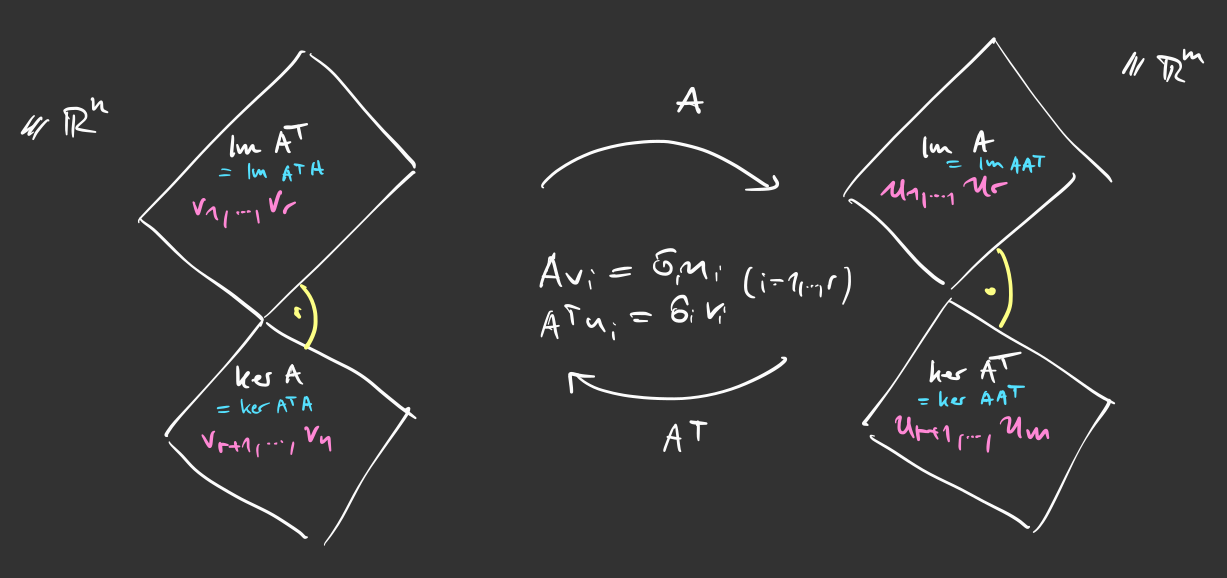
\includegraphics[width=0.6\linewidth]{svd-bigpic-la}
\end{center}

}
\end{frame}
}


%\begin{frame}
%~\\
%{
%2) Can we extend the singular vectors ...
%\begin{itemize}
%	\item [ a)]
%	... $v_1,\dots,v_r$ by $v_{r+1},\dots,v_n$ to form orthonormal basis of $\mathbb{R}^n$?
%	\item [ b)]
%	... $u_1,\dots,u_r$ by $u_{r+1},\dots,u_m$ to form orthonormal basis of $\mathbb{R}^m$?
%\end{itemize}
%\begin{itemize}
%	\item [ a)]
%	$v\in\text{ker}A=\text{ker}A^\top A~~\Rightarrow~~Av=0=0\cdot u~~\forall u\in\mathbb{R}^m$
%	\item [ b)]
%	$u\in\text{ker}A^\top =\text{ker}AA^\top ~~\Rightarrow~~A^\top u=0=0\cdot v~~\forall v\in\mathbb{R}^n$
%\end{itemize}
%$\Rightarrow$ Such $u\in\text{ker}A^\top $ and $v\in\text{ker}A$ can be considered singular vectors to the singular value 0.
%\begin{itemize}
%	\item [ a)]
%	For $i=1,\dots,r:~v_i=\frac{1}{\sigma_i}A^\top u_i~~\Rightarrow~~v_i\in\text{Im}A^\top =(\text{ker}A)^\bot$
%	\item [ b)]
%	$i=1,\dots,r:~u_i=\frac{1}{\sigma_i}Av_i~~\Rightarrow~~u_i\in\text{Im}A=(\text{ker}A^\top )^\bot$
%\end{itemize}
%Thus: $v\in\text{ker}A~(u\in\text{ker}A^\top )~~\Leftrightarrow~~v~(u)$ is orthogonal to all $v_1,\dots,v_r~(u_1,\dots,u_r)$\\
%\begin{columns}
%\begin{column}{.5\textwidth}
%	\begin{align*}
%	&v\in\text{ker}A\\
%	\Leftrightarrow~~&Av=0\\
%	\Leftrightarrow~~&U_r\Sigma_rV_r^\top v=0\\
%	\stackrel{U_r\Sigma_r \text{inj.}}{\Leftrightarrow}~~&V_r^\top v=0\\
%	\Leftrightarrow~~&\begin{pmatrix}
%	v_1^\top v\\\vdots\\v_r^\top v
%	\end{pmatrix}=\begin{pmatrix}
%	0\\\vdots\\0
%	\end{pmatrix}\\
%	\Leftrightarrow~~&v~\text{orthogonal to all}~v_1,\dots,v_r\\
%	\Leftrightarrow~~&v\in(\text{Im}V_r)^\bot=\text{ker}V_r^\top \\
%	\text{All in all:}~&\text{ker}A=\text{ker}V_r^\top 
%	\end{align*}
%\end{column}
%\begin{column}{.5\textwidth}
%	\begin{align*}
%	&u\in\text{ker}A^\top \\
%	\Leftrightarrow~~&A^\top u=0\\
%	\Leftrightarrow~~&V_r\Sigma_rU_r^\top u=0\\
%	\stackrel{V_r\Sigma_r \text{inj.}}{\Leftrightarrow}~~&U_r^\top u=0\\
%	\Leftrightarrow~~&\begin{pmatrix}
%	u_1^\top u\\\vdots\\u_r^\top u
%	\end{pmatrix}=\begin{pmatrix}
%	0\\\vdots\\0
%	\end{pmatrix}\\
%	\Leftrightarrow~~&u~\text{orthogonal to all}~u_1,\dots,u_r\\
%	\Leftrightarrow~~&u\in(\text{Im}U_r)^\bot=\text{ker}U_r^\top \\
%	\text{All in all:}~&\text{ker}A^\top =\text{ker}U_r^\top 
%	\end{align*}
%\end{column}
%\end{columns}
%}
%\end{frame}

%\begin{frame}
%~\\
%{
%3) How to find orthonormal basis for ker$A$ (ker$A^\top $):
%\begin{itemize}
%	\item [ a)]
%	w.l.o.g. assume $r<n$: (otherwise: ker$A$ = ker$V_n^\top  = \{0\}$)\\
%	For $i=r+1,\dots,n:$\\
%	\hspace{1cm}Find $\tilde{v}_i\in\text{ker}V_{i-1}^\top \setminus\{0\}~~~\leftarrow\text{This implies:}~\tilde{v}_{r+i}\in\text{ker}A~\text{and}~\tilde{v}_{r+i}^\top v_{r+j}~\forall j<i$\\
%	\hspace{1cm}Set $v_i=\frac{\tilde{v}_i}{\|\tilde{v}_i\|}$\\
%	\hspace{1cm}Set $V_i:=\left(V_{i-1}\lvert \begin{matrix}|\\v_i\\|\end{matrix}\right)~~~\leftarrow$ add column to $V_r$
%	\item [ b)]
%	w.l.o.g. assume $r<m$: (otherwise: ker$A^\top $ = ker$U_n^\top  = \{0\}$)\\
%	For $i=r+1,\dots,m:$\\
%	\hspace{1cm}Find $\tilde{u}_i\in\text{ker}U_{i-1}^\top \setminus\{0\}$\\
%	\hspace{1cm}Set $u_i=\frac{\tilde{u}_i}{\|\tilde{u}_i\|}$\\
%	\hspace{1cm}Set $U_i:=\left(U_{i-1}\lvert \begin{matrix}|\\u_i\\|\end{matrix}\right)$
%\end{itemize}
%
%}
%\end{frame}



\begin{frame}
	~\\
{\bf Summary and Remarks} \small
%$$A = U\Sigma V $$
$$
		A = \begin{pmatrix}
		|&&|&|&&|\\
		u_1&\cdots&u_r&u_{r+1}&\cdots&u_m\\
		|&&|&|&&|
		\end{pmatrix} 	\left(\begin{array}{ccc|ccc}
		\sigma_1&&&&\vdots&\\
		&\ddots&&\cdots&0&\cdots\\
		&&\sigma_r&&\vdots&\\\hline
		&\vdots&&&\vdots&\\
		\cdots&0&\cdots&\cdots&0&\cdots\\
		&\vdots&&&\vdots&
		\end{array}\right)  \begin{pmatrix}
		-&v_1&-\\
		~&\vdots&~\\
		-&v_r&-\\
		-&v_{r+1}&-\\
		~&\vdots&~\\
		-&v_n&-
		\end{pmatrix}
$$
\begin{itemize}
\item we can show $\im(A)  =  \spann(u_1,\ldots, u_r)$ and $\ker(A) = \spann(v_{r+1},\ldots, v_n)$, in particular
$$ {\color{satzrot}\rank(A) = r}$$
\item columns of $V$ are orthonormal eigenvectors of $A^\top A \in \Rnn$ and
$A^\top A = V (\Sigma^\top \Sigma )V^\top $
\item columns of $U$ are orthonormal eigenvectors of $AA^\top  \in \Rmm$
and
$AA^\top  = U (\Sigma \Sigma^\top ) U^\top $
\item $\sigma_1^2$ to $\sigma_r^2$ are the shared positive eigenvalues of both $A^\top A$ and $AA^\top $
\item an SVD of the transpose $A^\top$ is easily found by
 $$A^\top = (U \Sigma V^\top)^\top = V \Sigma^\top U^\top $$
\item for square matrices singular values and eigenvalues are different in general, take for example $A = -I$
\item however, for symmetric matrices $A=Q \Lambda Q^\top$, the singular values are the absolute values of the eigenvalues, i.e., $\sigma_i=\sqrt{\lambda_i^2}$ ~~(see exercises)
\end{itemize}
\end{frame}

\begin{frame}
\begin{example}[SVD by hand]\label{ex:SVDbyHand}
	~\\~\\
\Hide{	
	$A =\begin{bmatrix}
	3 & 2\\
	2 & 3\\
	2 & -2
	\end{bmatrix} $, 
	$A^\top  = \begin{bmatrix}
	3 & 2 & 2 \\
	2 & 3 & -2
	\end{bmatrix}$
	$$A^\top  A = \begin{bmatrix}
	3 & 2 & 2 \\
	2 & 3 & -2
	\end{bmatrix} \begin{bmatrix}
	3 & 2\\
	2 & 3\\
	2 & -2
	\end{bmatrix} = \begin{bmatrix}
	17 & 8\\
	8 & 17
	\end{bmatrix}$$
	\begin{itemize} 
		\item
		Compute eigenvalues of $A^\top A$:
		\begin{align*}
		&0\stackrel{!}{=}\det (A^\top A - \lambda I) = \text{det}\begin{pmatrix}
		17-\lambda&8\\8&17-\lambda
		\end{pmatrix} = (17-\lambda)^2 -64\\
		\Leftrightarrow~~& 17-\lambda = \pm 8\\
		\Leftrightarrow~~& \lambda = 17 \pm 8\\
		\Leftrightarrow~~& \lambda_1 = 25, \lambda_2 = 9
		\end{align*}
		\item
		Compute corresponding normalized eigenvectors:
		\begin{itemize}
			\item [a)]
			$(A^\top A-\lambda_1 I)v_1 =  \begin{pmatrix}
				-8 & 8\\
				8 & -8
			\end{pmatrix}v_1\stackrel{!}{=}0~~\Rightarrow~~v_1=\frac{1}{\sqrt{2}}\begin{pmatrix}1\\1\end{pmatrix}$
			\item [b)]
			$(A^\top A-\lambda_2 I)v_2 =  \begin{pmatrix}
			8 & 8\\
			8 & 8
			\end{pmatrix}v_2\stackrel{!}{=}0~~\Rightarrow~~v_2=\frac{1}{\sqrt{2}}\begin{pmatrix}1\\-1\end{pmatrix}$
		\end{itemize}
	\end{itemize}
}
\end{example}

\end{frame}

\begin{frame}
\Hide{~\\
\begin{itemize}
	\item Compute left singular vectors:~\\
	\begin{columns}
		\begin{column}{.5\textwidth}
			\begin{align*}
			\sigma_1&:=\sqrt{\lambda_1}=5,\\
			u_1&:=\frac{1}{\sigma_1}Av_1\\
			&=\frac{1}{5}\frac{1}{\sqrt{2}}\begin{pmatrix}
			3&2\\2&3\\2&-2
			\end{pmatrix}\begin{pmatrix}
			1\\1
			\end{pmatrix}\\
			&=\frac{1}{5\sqrt{2}}\begin{pmatrix}
			5\\5\\0
			\end{pmatrix}\\
			&=\frac{1}{\sqrt{2}}\begin{pmatrix}
			1\\1\\0
			\end{pmatrix}
			\end{align*}
		\end{column}
		%
		\begin{column}{.5\textwidth}
			\begin{align*}
			\sigma_2&:=\sqrt{\lambda_2}=3,\\
			u_2&:=\frac{1}{\sigma_2}Av_2\\
			&=\frac{1}{3}\frac{1}{\sqrt{2}}\begin{pmatrix}
			3&2\\2&3\\2&-2
			\end{pmatrix}\begin{pmatrix}
			1\\-1
			\end{pmatrix}\\
			&=\frac{1}{3\sqrt{2}}\begin{pmatrix}
			1\\-1\\4
			\end{pmatrix}
			\end{align*}
		\end{column}
	\end{columns}
~\\~\\
Find $u_3\in$ ker($A^\top $):
\begin{align*}
A^\top u_3=\begin{pmatrix}
3&2&2\\2&3&-2
\end{pmatrix}\begin{pmatrix}
u_3^1\\u_3^2\\u_3^3
\end{pmatrix}=\begin{pmatrix}
0\\0
\end{pmatrix}\\
u_3=\frac{1}{3}\begin{pmatrix}
2\\-2\\-1
\end{pmatrix}
\end{align*}
\end{itemize}
}
\end{frame} 

\begin{frame}
~\\
\Hide{
All in all:
\begin{align*}
V&=\begin{pmatrix}
|&|\\v_1&v_2\\|&|
\end{pmatrix}
=\frac{1}{\sqrt{2}}\begin{pmatrix}
1&1\\1&-1
\end{pmatrix} \in\mathbb{R}^{n\times n}=\mathbb{R}^{2\times 2}\\
U&=\begin{pmatrix}
|&|&|\\u_1&u_2&u_3\\|&|&|
\end{pmatrix}
=\begin{pmatrix}
\frac{1}{\sqrt{2}} & \frac{1}{3\sqrt{2}} & \frac{2}{3}\\
\frac{1}{\sqrt{2}} & -\frac{1}{3\sqrt{2}} & -\frac{2}{3}\\
0 & \frac{4}{3\sqrt{2}} & -\frac{1}{3}
\end{pmatrix} \in\mathbb{R}^{m\times m}=\mathbb{R}^{3\times 3}\\
\Sigma &=\begin{pmatrix}
\sigma_1&0\\0&\sigma_2\\0&0
\end{pmatrix}
=\begin{pmatrix}
5&0\\0&3\\0&0
\end{pmatrix} \in\mathbb{R}^{m\times n}=\mathbb{R}^{3\times 2}\\
&\\
\Rightarrow~~A=U\Sigma V^\top 
\end{align*}
}
\end{frame}



\elomath{
\begin{frame}
~\\
\textbf{Example:} rank-1 pieces\\~\\
Let $x\in\mathbb{R}^m\setminus\{0\}$ and $y\in\mathbb{R}^n\setminus\{0\}$, then
$$
A:=xy^\top =\begin{pmatrix}
x_1\\\vdots\\x_m
\end{pmatrix} (y_1,\dots,y_n)
=\begin{pmatrix}
|&&|\\y_1x&\cdots&y_nx\\|&&|
\end{pmatrix}\in\mathbb{R}^{m\times n}.
$$
What is the SVD of $A$?\\~\\
\Hide{
$$
A^\top A = (xy^\top )^\top xy^\top =y\underbrace{x^\top x}_{=\|x\|^2}y^\top =\|x\|^2yy^\top 
$$
Compute eigenpairs: We find $A^\top Ay=\|x\|^2y\underbrace{y^\top y}_{=\|y\|^2}=\|x\|^2 \|y\|^2y$\\
$v_1:=\frac{y}{\|y\|}$ is eigenvector to the eigenvalue $\lambda_1:=\|x\|^2\|y\|^2$\\
Set $$\sigma_1:=\sqrt{\lambda_1}\stackrel{(\neq0,\text{since}x\neq0\neq y)}{=}\|x\|\|y\|$$ and $$u_1:=\frac{1}{\sigma_1}Av_1=\frac{1}{\|x\|\|y\|}xy^\top \frac{y}{\|y\|}=\frac{x}{\|x\|}$$ then
$$
A=U\Sigma V^\top =\frac{x}{\|x\|}(\|x\|\|y\|)\frac{y^\top }{\|y\|}=xy^\top ~\checkmark~~~~(\rightarrow r=1,~\text{thus rank}(A)=1)
$$
}
\end{frame}
}


\begin{frame}
	\Subsection{The Geometry of the SVD}
	[Compare to the geometry of the eigendecomposition]\\
	\Hide{ 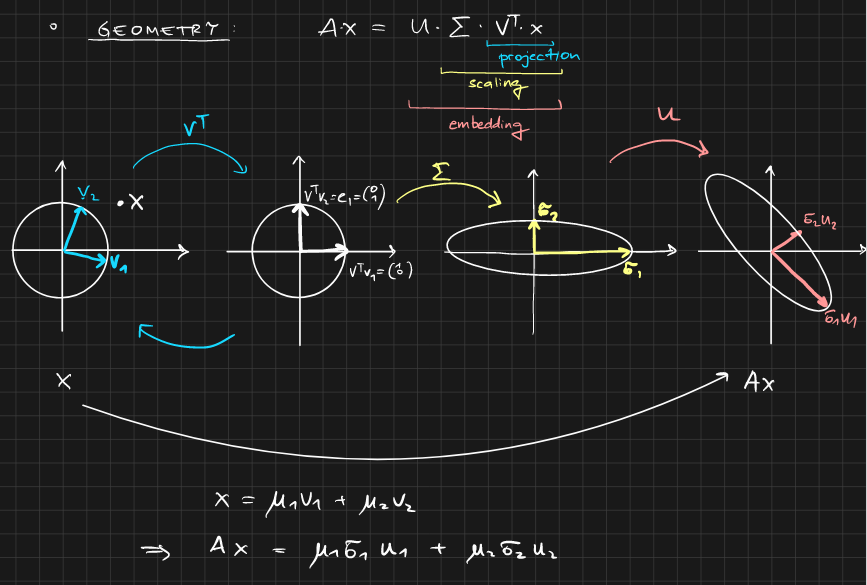
\includegraphics[width=.85\textwidth]{SVD_Recap}
	~\\ \footnotesize
\begin{itemize}
	\item The orthonormal bases $V$ and $U$ are connected via $Av_j = \sigma_j u_j$.
	\item Using these orthonormal bases, one can regard \textit{any} matrix as a diagonal matrix.
\end{itemize}
}
\end{frame}


%MATRIX CONDITION AND RANK
\begin{frame}
\Subsection{Matrix condition and rank}
~\\
\textbf{\color{header}Situation:}\\~\\
 Let $A = U\Sigma V^\top  \in \R^{n\times n}$ be invertible (i.e., $\sigma_i \neq 0~ \forall i$) and assume we want to solve $Ax=b$. We also assume that the data is corrupted $\tilde{b} = b+\Delta b$ by some error $\Delta b$.\\~\\
~~$\Rightarrow$~We obtain a perturbed solution $\tilde{x} = x + \Delta x$ with $\Delta x=A^{-1}\Delta b$.\\~\\
\textbf{\color{header}Question:}\\~\\ How severe is the propagation of \textit{data error} $\Delta b$ to the resulting \textit{solution error} $\Delta x$?\\
~~~ $\rightarrow$ Singular (eigen-) values give us this information!~\\
\Hide{
\begin{align*}
b=Ax &\Rightarrow \|b\|_2=\|Ax\|_2=\|U\Sigma V^\top x\|_2=\|\Sigma V^\top x\|_2=\|\Sigma_{j=1}^r\sigma_j v_j^\top x\|_2\le \sigma_1 \|V^\top x\|_2=\sigma_1\|x\|_2\\[0.2cm]
\Delta x=A^{-1}\Delta b&\Rightarrow \|\Delta x\|_2=\|A^{-1}\Delta b\|_2=\|V\Sigma^{-1}U^\top \Delta b\|_2=\|\Sigma^{-1}U^\top \Delta b\|_2\le\frac{1}{\sigma_n}\|\Delta b\|_2\\[0.2cm]
&\Rightarrow  \frac{\|\Delta x\|_2}{\|x\|_2} \le \frac{1}{\sigma_n}\frac{\|\Delta b\|_2}{\|x\|_2} \le \frac{\sigma_1}{\sigma_n}\frac{\|\Delta b\|_2}{\|b\|_2}
\end{align*}
}
\end{frame}

\begin{frame}
	~\\
\begin{definition}[Condition number]\label{def:conditionnumber}
Let $A\in \R^{n\times n}$ be a matrix. Then we call 
$$\text{cond}_2(A):=\frac{\max\{\sigma_i\}}{\min\{\sigma_i\}}$$ 
the \textbf{condition number} of the matrix $A$.
\end{definition}
~\\~\\
\textbf{Special Case:} Symmetric Matrices { (exercise)}\\[9pt]
Let $A\in\R^{n\times n}$ be a real symmetric matrix, then $$\text{cond}_2(A)=\frac{\max\{|\lambda|\colon \lambda\in\sigma{(A)}\}}{\min\{|\lambda|\colon \lambda\in\sigma{(A)}\}}.$$
	~\\~\\
\textbf{Remark:}\\~\\ If some of the singular values are actually zero or close to zero, the condition number is (almost) $\infty$. In this case, we cannot trust any numerical solver (for $Ax=b$) in finite precision, as errors in the data $b$ (e.g., also due to rounding errors) may severely propagate to the computed solution $x$.\\~\\ We also call such matrices \textit{rank deficient}.
\end{frame}




%%%%%%%%%%%%%%%%%%%%%%%%%%%%%%%%%%%%%%%%%%%%%%%%%
% APPLICATION SVD




%========= BEST APPROXIMATION PROPERTY
\begin{frame}
\Subsection{The Truncated SVD and its Best Approximation Property}
%Consider a matrix $A \in \R^{m \times n}$ with SVD $A=U\Sigma V^\top$ and $r:= \text{rank}(A)$ so that
%$$
%\Sigma =		\left[\begin{array}{ccc|ccc}
%\sigma_1&&&&\vdots&\\
%&\ddots&&\cdots&0&\cdots\\
%&&\sigma_r&&\vdots&\\\hline
%&\vdots&&&\vdots&\\
%\cdots&0&\cdots&\cdots&0&\cdots\\
%&\vdots&&&\vdots&
%\end{array}\right].
%$$
~\\
\textbf{\color{header}Motivation:}\\
Let the singular values be sorted $\sigma_1 \geq \ldots \geq \sigma_r > 0$, $r := \text{rank}(A)$, then the reduced SVD reads as 
$$A = \sigma_1 u_1 v_1^\top  +\sigma_2 u_2 v_2^\top  + \cdots+\sigma_i u_i v_i^\top  +\cdots + \sigma_{r-1} u_{r-1} v_{r-1}^\top  + \sigma_{r} u_r v_r^\top    $$
If a $\sigma_i$ is small, then the matrix $u_i v_i^\top $ does not contribute much to $A$, and similarly for $\sigma_{i+1},\ldots, \sigma_r$.\\~\\
What about leaving them out?
~\\~\\~\\
This gives rise to the following definition:\vspace{-0.1cm}
\begin{defi}[Truncated SVD]
	Let $A = U\Sigma V^\top  \in \Rmn$. For $k <r:= \text{rank}(A)$ define $\Sigma_k:=\text{diag}(\sigma_1,\ldots,\sigma_k) \in \R^{k \times k}$, $U_k := [u_1,\ldots,u_k]\in \R^{m \times k}$ and $V_k:= [v_1,\ldots,v_k]\in \R^{n \times k}$. Then $$A_k := U \text{diag}(\sigma_1,\ldots,\sigma_k,0\ldots,0)V^\top  = U_k \Sigma_k V_k^\top $$ is called \textbf{truncated SVD of $A$}.
\end{defi}
We \text{observe} that $$\text{rank}(A_k) = k,$$ which is why $A_k$ is also called \textit{rank-$k$-approximation of $A$}.\\[5pt]
\end{frame}

\begin{frame}
\textbf{\color{header}Question:} Leaving out some rank-1 summands, how much do we deviate from the original matrix?
\\~\\ 
With other words: In which sense does $A_k \in \R^{m\times n}$ \textit{approximate} $A \in \R^{m\times n}$?
\\~\\
We first need to quantify the distance between matrices, i.e., we need a \textit{norm} for matrices in $\Rmn$!\\~\\
Here we consider the so--called Frobenius norm:\\ If we reshape a matrix $A \in \Rmn$ into a vector $v\in \R^{m\cdot n}$  (e.g., $v_{[(j-1)\cdot m+i]}:=a_{ij}$), then we can use our norms for vectors, e.g.,
$$\|A\|_F:=\|v\|_2.$$
~\\
This is precisely: \vspace{-0.1cm}
\begin{definition}[Frobenius norm]
	For any matrix $A\in\R^{m\times n}$, the \textbf{Frobenius norm} is defined as
	$$
	\|A\|_F:=\sqrt{\sum\limits_{i=1}^m\sum\limits_{j=1}^na_{ij}^2}.
	$$
\end{definition}
~\\
Exercise:
\begin{itemize}
\item One can show that $$\|A\|_F^2=\text{tr}(A^\top A),$$ where tr:=``trace'' denotes the sum of the diagonal entries.\\~\\
\item Using this fact, for $A=U\Sigma V^\top$ with $r=\rank(A)$ we also find
$$\|A\|_F^2=\sum_{i=1}^{r}\sigma_i^2.$$ 
\end{itemize}
\end{frame}

\begin{frame}
	~\\~\\
Finally, the truncated SVD satisfies a best approximation property:\vspace{-0.1cm}
\begin{theorem}[Eckart-Young-Mirsky]\label{Eckart-Young-Mirsky} Let $A\in\R^{m\times n}$ with SVD $A=U\Sigma V^\top$ and let $k\le \text{rank}(A)$. Then, the truncated SVD $A_k$ is the best approximation in the Frobenius norm among all matrices with rank $k$, i.e. 
	\[\|A-A_k\|_F\le \|A-B\|_F\, ,\quad\forall B\in\R^{m\times n},\text{rank}(B)=k.
	\]
\end{theorem}
~\\
	\text{In words:}~\\
	\begin{center}
		\textbf{\large\textit{Among all matrices with rank $k$, the truncated SVD is closest to $A$.}}
	\end{center}
~\\
\Hide{\begin{proof}
	We use the so-called Weyl inequality (see \eqref{Weyl} below): For matrices $C,D\in\R^{m\times n}$ with decreasingly ordered singular values, we denote by $\sigma_i(C),\sigma_i(C),\sigma_i(C+D)$ the $i$-th singular value of the respective matrix. Then Weyl's inequality gives us the relation
	\begin{equation}\label{Weyl}
	\sigma_{i+\ell-1}(C+D)\le \sigma_i(C)+\sigma_\ell(D), \text{ with }i,\ell, i+\ell-1\in\{1,...,p\}\, ,\ p:=\min\{m,n\}.
	\end{equation}
	We assume rank$(B)=k$, which results in $\sigma_l(B)=0$ for $l>k$ and thus we conclude from Weyl's inequality (\ref{Weyl}) for $C:=A-B, D:= B, \ell:=k+1$ that
	\begin{align*}
	\sigma_{i+k}(A)&\le\sigma_i(A-B)+\sigma_{k+1}(B)=\sigma_i(A-B) \text{  for }i=1,...,p-k\\
	\Rightarrow \|A-B\|_F^2&=\sum_{i=1}^{p}\sigma_i(A-B)^2\ge\sum_{i=1}^{p-k}\sigma_i(A-B)^2\ge\sum_{i=k+1}^{p}\sigma_i(A)^2=\|A-A_k\|_F^2
	\end{align*}
	for all $B$ with rank$(B)=k$.	
\end{proof}	 }
\end{frame}


%========= Eckart-Young-Mirsky
%\begin{frame}
%\begin{theorem}[Eckart-Young-Mirsky]\label{Eckart-Young-Mirsky} Let $A\in\R^{m\times n}$ be a real matrix with SVD $A=U\Sigma V^\top$ and $k\le\min\{m,n\}$. Then, the truncated SVD $A_k$ is the best approximation in the Frobenius norm among all matrices with rank $k$, i.e. 
%	\[\|A-A_K\|_F\le \|A-B\|_F\, ,\quad\forall B\in\R^{m\times n},\text{ rank}(B)=k
%	\]
%\end{theorem}

%\end{frame}

%========= REMARKS
%\begin{frame}
%\begin{re} ~\\[-14pt]
%	\ite
%	\item We'll see below that $\sigma_1(A)$ itself is already a norm. Obviously the same theorem holds also for this norm instead of the Frobenius norm---in the proof, we just have to choose $i=1$ only.
%	\item Warning: publications dealing with low rank approximations sometimes call a decomposition $A=U\Sigma V^\top$ an ``SVD'', even in the case, when neither $U$ nor $V$ are orthogonal matrices. Just make sure to read the fine print in all those publications.
%	\eti
%\end{re}
%\end{frame}

%IMAGE COMPRESSION
\begin{frame}
\Subsubsection{Image and Data Compression}
~\\
\begin{minipage}[c]{0.6\textwidth}
	
 	\begin{tikzpicture}
\node[inner sep=0pt] (dina0) at (0,0)
{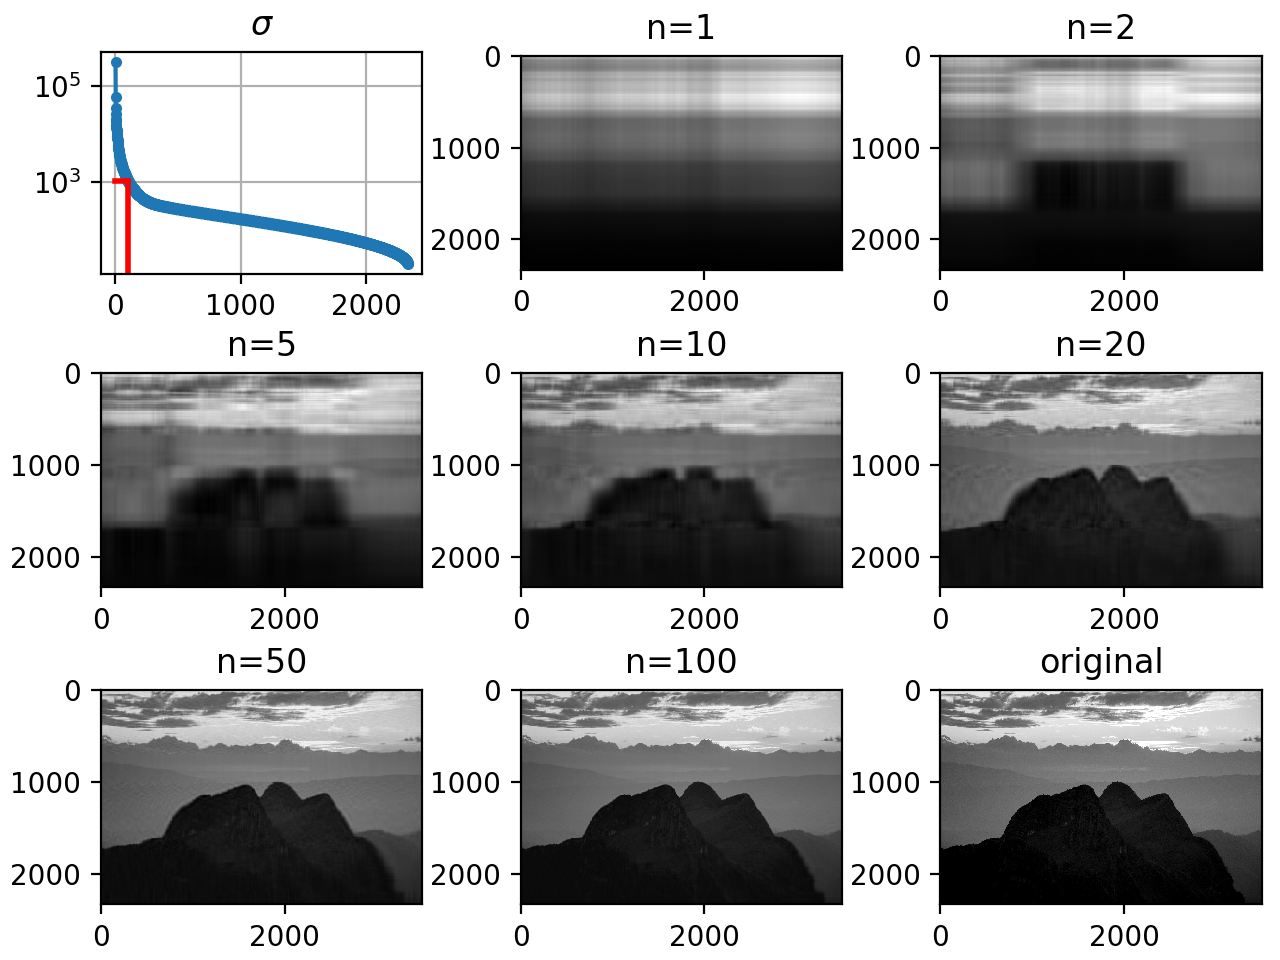
\includegraphics[width=\textwidth]{6_svd_mountain.png}};
\end{tikzpicture}		
\end{minipage}
\begin{minipage}[c]{0.001\textwidth}
	\
\end{minipage}
\begin{minipage}[c]{0.35\textwidth}
	$3500\times2333$ greyscale image is interpreted as matrix $$A\in[0,1]^{3500\times2333}.$$ 
	The singular values are shown in the figure with the title ``$\sigma$''.\\ 
	The reconstructed image with the first 100 singular values only, i.e.,
	$$A_{100}:=U\text{diag}(\sigma_1,\ldots,\sigma_{100},0,\ldots ,0)V^\top$$ 
	is quite close to the original image but takes only
	\[
	\frac{3500\cdot 100+100+100\cdot 2333}{3500\cdot 2333}\approx 7\%
	\]
	of the storage space.
\end{minipage}
~\\~\\
Note: The storage of $A_k$ in general is $k \cdot (m + 1 + n)$.\\~\\
Note: The same data compression can be performed with any matrix --- and similarly with tensors.
\end{frame}

%========= PYTHON CODE for IMAGING
%\begin{frame}
%\hfill{\footnotesize The {\tt Python3} listing:}\hspace{0.4\textwidth}
%\vspace{-0.2cm}
%\lstinputlisting[lastline=24]{python_examples/6_svd_image.py}
%\end{frame}


%PCA
\begin{frame}
	\Subsubsection{Principal Component Analysis (PCA)}
	\Hide{
	%\textbf{Problem formulation:}\\
	% Observation vectors $\{v_1,\ldots,v_n\}\subset \R^m$ around zero, i.e.~$\sum_{i=1}^nv_i=0$, are to be represented as vectors $\{w_1,\ldots,w_n\}\subset \R^k$ in a much lower dimensional space, i.e., $k < m$, as accurately as possible. Accuracy is measured in $\|\cdot\|_2$.\\
	%A Matrix $Z\in \R^{m\times k}$ with orthogonal columns gives us an embedding of $\R^k$ into $\R^m$ and its transpose a projection  of $\R^m$ into $\R^k$. Thus, we are looking for such a matrix $Z$ which solves
	%\[
	%\min_Z\sum_{i=1}^n\|v_i-ZZ^\top v_i\|^2_2=\|A-ZZ^\top A\|^2_F
	%\]
	%with  $A:=[v_1,\ldots,v_n]$.\\[5pt]
	%\textbf{Solution:}\\ Since $\text{rank}(ZZ^\top A) = k$, we know the solution already from Theorem \ref{Eckart-Young-Mirsky} as
	%$$ZZ^\top A=A_k=U\text{diag}(\sigma_1,\ldots,\sigma_k,0,\ldots,0) V^\top,$$ 
	%such that $Z=U_k:=[u_1,\ldots,u_k]$.\\
	%Therefore, the lower dimensional representation vectors are 
	%$$\{w_1=U_k^\top v_1,\ldots,w_n=U_k^\top v_n\}.$$ 
	%The so-called \textbf{``principal components''} are the lines associated with the columns of $U_k$, i.e., the sets $$\{\alpha u_i\spy\alpha\in\R\}~~~\text{for}~~~ i=1,\ldots ,k.$$
	\underline{Situation:}\\
	$n$ measurements / samples (e.g., questioning $n$ persons)\\
	$m$ features / variables (e.g., height and weight)\\~\\
	\underline{Example:}\\
	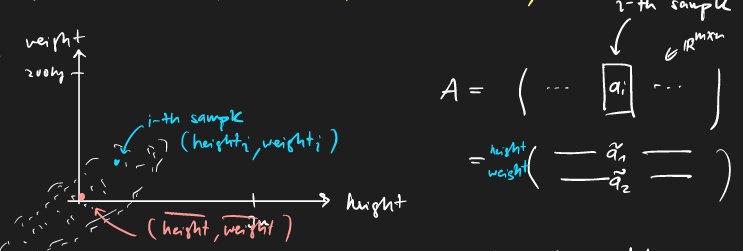
\includegraphics[width=.75\textwidth]{PCA_Example}~\\
	Without loss of generality we can center the data by substracting the mean from each sample\\~\\
	\underline{Observation:}\\
	Height and weight are proportional in some sense (i.e., they correlate), however there is some spread/variance.\\~\\
	\underline{Aim:}\\
	Can we explain ``most'' of the variance with a lower dimensional subspace?\\
	(In the example above, e.g., a line may capture most of the variance)
}
\end{frame}

\begin{frame}
	~\\
	\Hide{
		\underline{More on the statistics:} (Var$(X)=E(X-E(X))^2$)~\\
	\begin{center}
		statistical	variance = ``normalized'' sum of squared distances from the mean
	\end{center}
		\begin{align*}
		\text{statistical variance in height}~=~\frac{1}{n-1}\sum_{i=1}^n(\text{height}_i-\underbrace{\overline{\text{height}}}_{\text{w.l.o.g.}=0})^2
		=~\frac{1}{n-1}\sum_{i=1}^n\widetilde{\text{height}}_i^2~=~\frac{1}{n-1}\tilde{a}_1^T\tilde{a}_1
		\end{align*}
		\begin{align*} 
		A=\begin{matrix}
		m~\text{feats}&~\\
		\downarrow&\begin{pmatrix}
		-\tilde{a}_1-\\-\tilde{a}_2-
		\end{pmatrix}\\
		~&\overrightarrow{n~\text{people}}
		\end{matrix}
		~~\leftarrow~\text{centered}~~\begin{matrix}
		\text{height measurements}\\
		\text{weight measurements}
		\end{matrix}
		\end{align*}
		Then:
		\begin{align*}
		\frac{1}{n-1}AA^T=\frac{1}{n-1}\begin{pmatrix}
		-\tilde{a}_1-\\-\tilde{a}_2-
		\end{pmatrix}\begin{pmatrix}
		|&|\\\tilde{a}_1&\tilde{a}_2\\|&|
		\end{pmatrix}
		=\frac{1}{n-1}\begin{pmatrix}
		\tilde{a}_1^T\tilde{a}_1&\tilde{a}_1^T\tilde{a}_2\\
		\tilde{a}_2^T\tilde{a}_1&\tilde{a}_2^T\tilde{a}_2
		\end{pmatrix}\\
		(\text{diagonals: variances, off-diagonals: co-variance})
		\end{align*}
	}
\end{frame}

\begin{frame}
	~\\
\Hide{
		\underline{Using SVD:} $A=U\Sigma V^T$
		$$
		\frac{1}{n-1}AA^T=\frac{1}{n-1}U\begin{pmatrix}
		\sigma_1^2&~&0\\~&\ddots&~\\0&~&\sigma_r^2
		\end{pmatrix}U^T=\frac{1}{n-1}\sum_{i=1}^r \sigma_i^2u_iu_i^T
		$$
		Thus, the first few summands explain most of $AA^T$, i.e., the variance\\
		The singular vectors $u_1,\dots,u_r$ are called principal components in this setting.\\
		(\underline{Remark:} $\|A\|_F=\text{tr}(AA^T)=\sum_{i=1}^m\tilde{a}_i^T\tilde{a}_i$ = sum of variances)\\
		~\\
		\underline{Now to the geometry of the SVD:}
		$$
		A=\begin{matrix}
		m~\text{feats}&\underrightarrow{n~\text{samples}}\\
		\downarrow&\begin{pmatrix}
		|&~&|&~&|\\
		a_1&\cdots&a_i&\cdots&a_n\\
		|&~&|&~&|
		\end{pmatrix}
		\end{matrix}
		=U\textcolor{cyan}{\Sigma V^T}
		=\underbrace{\begin{pmatrix}
			|&~&|\\u_1&\cdots&u_m\\|&~&|
			\end{pmatrix}}_{\text{orthonormal basis}}
		\underbrace{\textcolor{cyan}{(\Sigma V^T)}}_{\text{coordinates of}~a_i~\text{in terms of this basis}}
		$$
		Thus, each sample $a_i\in\mathbb{R}^m$ is a linear combination of $u_1,\dots,u_m$ with coefficients $(\Sigma V^T)_i=c_i=\begin{pmatrix}
		c_1^i\\c_2^i
		\end{pmatrix}$\\
	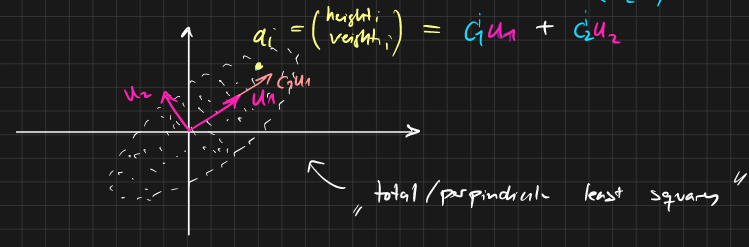
\includegraphics[width=0.5\textwidth]{SVD_Geometry}
	}
\end{frame}

\begin{frame}
	~\\
\Hide{
		The speciality about the particular orthonormal system $u_1,\dots,u_m~(m=2)$ is this:\\
		~\\
		If we only take the first $u_1,\dots,u_k~(k=1)$ then among all orthonormal systems which are composed of $k$ vectors, these give the best approximation to $A$ (= the measurements) in the $\|\cdot\|_F$-sense.
	}
\end{frame}
 
\begin{frame}
	\Subsubsection{Pseudoinverses}
	With the help of the SVD one can define a generalized concept of an inverse matrix, called the \textit{pseudoinverse}. This is closely related to the minimum-norm least-squares solution, so that we postpone a discussion to the section on least squares. 
\end{frame}



%%%%
% NUMERICAL COMPUTATION OF THE SVD
%%%%
\begin{frame}
\Subsection{Numerical Computation of the SVD}
\Hide{Let us write equation \eqref{eq:SVDstart} in matrix form:\\
$$
\begin{pmatrix}
	0&A\\A^\top &0
\end{pmatrix}
\cdot
\begin{pmatrix}
 u\\v
\end{pmatrix}
=
\begin{pmatrix}
 Av\\ A^\top u
\end{pmatrix}
=
\begin{pmatrix}
\sigma u\\ \sigma v
\end{pmatrix}
=
\sigma\begin{pmatrix}
 u\\ v
\end{pmatrix}.
$$
Then this reads as an eigenvalue problem for the symmetric matrix $S:=\begin{pmatrix}
0&A\\A^\top &0
\end{pmatrix}$.\\~\\
Thus we already identify $r$ eigenpairs for $S$, namely, 
$$(\sigma_1,\begin{pmatrix}
u_1\\ v_1
\end{pmatrix}), \ldots, (\sigma_r,\begin{pmatrix}
u_r\\ v_r
\end{pmatrix}),$$ where $(\sigma_i,\begin{pmatrix}
u_i\\ v_i
\end{pmatrix})$ are the $r$ singular values and vectors of $A$, respectively.
~\\~\\
Also we easily find that 
$$(-\sigma_1,\begin{pmatrix}
-u_1\\ v_2
\end{pmatrix}), \ldots, (-\sigma_r,\begin{pmatrix}
-u_r\\ v_r
\end{pmatrix})$$
 are eigenpairs of $S$.\\ 
 For the remaining $(m-r)+(n-r)$ eigenpairs take orthonomal bases $u_{r+1},\ldots, u_m\in\text{ker}A^\top$ and $v_{r+1},\ldots, v_n\in\text{ker}A$, then the $(0,\begin{pmatrix}
	u_i\\ 0
\end{pmatrix})$ and $(0,\begin{pmatrix}
0\\ v_i
\end{pmatrix})$ give the remaining eigenpairs (with eigenvalue $0$).
 ~\\~\\
 Implications:\\
	$\rightarrow$ We can compute the SVD without computing $A^\top A$ or $AA^\top $.\\
	$\rightarrow$ Goes back to Gene Golub in the 1960s ($\rightarrow$ see his license plate)
}
\end{frame}
\begin{frame}
\Hide{~\\
	\textbf{Final Remark:}\\~\\
	 The SVD is a powerful tool and being able to compute it efficiently further facilitates, among others, the following:~\\
	\begin{itemize}
				\item standard method for computing matrix norms $\|A\|_F$ (or $\|A\|_2 := \sigma_1$)
		\item the best method for determining the rank of a matrix is to
		count the number of singular values greater than a judiciously chosen tolerance (note: the fundamental problem is distinguishing a small float which is prone to rounding errors from an actual zero!)
		\item most accurate method for finding an orthonormal
		basis of a range or a nullspace
		\item standards for computing low-rank	approximations w.r.t to $\|\cdot\|_F$
		\item ingredient in robust algorithms for least squares fitting via pseudoinverse
	\end{itemize}}
\end{frame}

